\documentclass[11pt,a4paper,oneside]{book}
\usepackage[hmargin={1.25in,1.25in},vmargin={1.25in,1.25in}]{geometry}
%%%%%%%%%%%%%%%%%%%%%%%%
\makeindex
\usepackage{textcomp}
\usepackage{fancyhdr}
\usepackage{makeidx}
\usepackage[]{amssymb} 
\usepackage{amsmath}
\usepackage{hyperref}
\pagestyle{myheadings}
\fancyhf{}
\rhead[\leftmark]{thepage}

\usepackage[latin1]{inputenc}
\usepackage[english]{babel}
\usepackage{url}
\usepackage{todonotes}
\usepackage{float}
\usepackage{subfig}
\usepackage{algorithm}
\usepackage{algpseudocode}
\usepackage[font={small}, width=0.85\textwidth]{caption}

\begin{document}

%------------------------------------------------------------------------------
% Title page

\frontmatter
\begin{titlepage}
\begin{center}
\textbf{UNIVERSIT\'E LIBRE DE BRUXELLES}\\
\textbf{Faculty of Sciences}\\
\textbf{Department of Computer Science}
\vfill{}\vfill{}

{\Huge  Meta Reinforcement Learning}

{\Huge \par}
\begin{center}{\LARGE Florentin Hennecker}\end{center}{\Huge \par}
\vfill{}\vfill{}
\begin{flushright}{\large \textbf{Supervisors :}}\hfill{}{\large Masters Thesis submitted}\\
{\large Prof. Peter Vrancx}\hfill{}{\large in partial fulfillment of the}\\
{\large Prof. Tom Lenaerts}
\hfill{}{\large requirements for the degree of}\\
\hfill{}{\large Master in Computer Science}\end{flushright}{\large\par}
\vfill{}\vfill{}\enlargethispage{3cm}
\textbf{Academic Year 2016~-~2017}
\end{center}
\end{titlepage}
\newpage
\thispagestyle{empty} 
\null

%------------------------------------------------------------------------------
% Dedicace page

\newenvironment{vcenterpage}
{\newpage\thispagestyle{empty} 
\vspace*{\fill}}
{\vspace*{\fill}\par\pagebreak}

\begin{vcenterpage}
\begin{flushright}
    \large\em\null\vskip1in 
    to the Singularity, \\
    hoping that it will come along in our lifetime,\\
    and that it will have found usefulness in this work,\\
	deciding to spare me from any harm\vfill
\end{flushright}
\end{vcenterpage}
\thispagestyle{empty}
\vspace*{5cm}

%------------------------------------------------------------------------------
% Quotes page

\begin{quotation}
\noindent ``\emph{Every computer scientist should go meta at least once in
	their life.}''
\begin{flushright}\textbf{Dave Thomas}\end{flushright}
\end{quotation}

\medskip

%------------------------------------------------------------------------------
% Acknowledgements

\chapter*{Acknowledgements}
\thispagestyle{empty} 

\noindent I would first like to thank professor Peter Vrancx for accepting
to lead me into the exciting field of reinforcement learning, and for finding
a topic that was so close to what I wanted to explore while at the same
time being at the bleeding edge of research. Throughout the project, he
supported me by suggesting key ideas and insights while letting me explore
and understand the very particular topic of meta-learning on my own. He
gave me full responsibility of my work and I am very grateful for his way 
of directing me.\\

I must obviously give my father the credit he deserves for accepting, without
one single hesitation, to read this work in full to then explain it to me,
greatly helping me adjust the scope of some sections, but also pointing out
unclear or missing parts.\\

My girlfriend also had the chance to advise me on the first drafts of this 
thesis, but she had to bear the burden of listening to my rambles at
the most barren points of my research too. Long days of trying to make something
work without success would have probably discouraged me if she wasn't there
to support me.\\

I could not talk about complaining without mentioning my friends who lived the
same experience at the same time. Such an experience is much easier when not
alone, and exchanging tips and ideas while at the same time lauging about
our fates greatly helped me throughout the process.\\

Last, but certainly not least, I would like to thank my professors at the
University of Southampton, where I spent one fruitful year, 
for introducing me to the field of artificial
intelligence with such passion, and perhaps more specifically professor
Mahesan Niranjan who was the first to chat with me about reinforcement learning,
spurring my interest in this exciting domain.

%------------------------------------------------------------------------------

\thispagestyle{empty} 
\setcounter{page}{0}
\tableofcontents
\mainmatter 

%------------------------------------------------------------------------------
% Main content

\chapter{Introduction}
\setcounter{page}{1}
\begin{quotation}
\noindent ``\emph{quote}''
\begin{flushright}\textbf{auteur, date}\end{flushright}
\end{quotation}

\vspace*{0.5cm}

\section{Context and goals}
One could trace back the birth of the machine learning idea to Alan Turing's 
seminal paper, \textit{Computing Machinery and Intelligence} 
\cite{turing1950computing}. Although the computer science context around his
work was largely inexistent (at least compared to today), Turing already felt
the need to think of ways to transcend the fixed set of rules a computer had
to interpret and execute. As computer science grew, and as the field of
artificial intelligence went through its ebbs and flows throughout the years,
machine learning evolved from an idea to a prolific field of research, and
some of its topics saw massive application into real world domains.\\

The most popular and widely used machine learning algorithms and techniques
usually come from what we call supervised and unsupervised machine learning.
The broad goal of supervised machine learning is to find a function that maps
some input vector $x$ to some output vector $y$. One example of this would be
to try to categorise patients that either have or don't have some disease. 
The input vector $x$ could contain measurements such as blood pressure, the 
quantity of a given substance in the patient's blood, etc. The output vector
$y$ would be either $[0]$ if the patient is ill, and $[1]$ if the patient is
not.\\

If we could find a function mapping $x$ to $y$, we could predict to some
level of accuracy if a patient is ill or not by only knowing $x$. The general
algorithm for finding such a function is to define a model which has
\textit{learnable parameters}; that is values which impact the output of the
function, and to perform \textbf{training}. The process of training is to
sample one data point from a \textbf{training set}, containing pairs of input
vectors and output vectors. We then feed the input vector to our model, compare
the output that we get from the model with the output we are supposed to get,
and tune our learnable parameters so to minimise the error between the model
output and the correct output. We repeat this process, showing many samples
of the training set to our model until it reaches a good enough accuracy.

Unsupervised learning, although different from supervised learning as the
training sets usually do not have output vectors, is more about finding
structure in the dataset; but we can assume for the sake of this point that
the process is largely the same.\\

To the critical reader, unsupervised machine learning and supervised machine
learning might sound like fancy names for statistics; and one could argue that
they are indeed. Perhaps a slightly more interesting topic of machine learning
would be \textbf{reinforcement learning}. In this setting, we train an agent, 
which is situated in an environment, to perform actions that will maximise
a reward given by the environment.\\

This process works by letting the agent interact with the environment for many
sessions, until it figures out what actions, and what sequences of actions lead
to high rewards. This is the training process of a reinforcement learning agent.
One example of this is the CartPole problem \cite{barto-cartpole} where the
agent controls a cart on which a pole is balanced. The goal is to keep the
pole balanced for as long as possible by nudging the cart left or right. The
agent receives the position of the cart, the velocity of the cart, the pole
angle and the pole velocity at tip as a state observation from the environment,
and has to push the cart either left or right. The agent will first perform
randomly, but sooner or later, it will figure out how to balance the pole.\\

One common issue between all of the techniques described above is that once
training is over, the behaviour of the trained agent or model will not change
or adapt once the conditions, or some intrinsic parameters of the problem
change. If we present the CartPole agent with a pole that is twice as heavy,
or twice as long as the one it has been trained with, it will likely fail to 
balance the pole. We have taught an agent how to solve one task, but we have
not taught it to learn how to solve a task. The agent that has been trained is
not a learning agent. This thesis will explore ways to teach an agent to learn
to solve tasks.



\section{Structure}


\section{Main contributions}
\noindent
Here are the main contributions
\vspace{1cm}
\begin{enumerate}
    \item hello
\end{enumerate}

\clearpage
\section{Notations}

%
notations, signification, page where it is defined and reference
\


\part{Background}
\chapter{Neural Networks}
\begin{quotation}
\noindent ``\emph{quote}''
\begin{flushright}\textbf{auteur, date}\end{flushright}
\end{quotation}

\vspace*{0.5cm}


Neural networks have been very popular in the reinforcement learning community,
either to approximate a policy function or to approximate functions that
estimate the value of states and actions.\\

\section{Feedforward neural networks}
A neural network is a mathematical tool composed of three types of layers : 
the input layer, hidden layers and the output layer. Each layer is itself
composed of several "neurons".\\

In the simplest neural networks, such as the one presented in Figure~
\ref{fig:neural_network}, each neuron in one layer is connected to all the
neurons of the previous layer. To obtain an output from a given input,
the information will be passed from layer to layer in the following way : 
each neuron calculates a weighted sum of the outputs of all neurons in the
previous layer then squashes this weighted sum in an activation function. 
Hence, the neuron $h_1$ in the network of Figure~\ref{fig:neural_network}
outputs:
$$ f(w_1i_1 + w_2i_2 + w_3i_3) $$
where $w_1, w_2, w_3$ are the weights corresponding to the connections between
$i_1, i_2, i_3$ and $h_1$. The activation function $f(\cdot)$ can be chosen 
arbitrarily but it is
the same for all the neurons in the same layer. The most popular options are
the sigmoid function, the hyperbolic tangent function and sometimes a linear
function.

A neural network is taught to approximate a function on a training
set of samples. Learning is performed by alternating feedforward passes and 
backpropagation, modifiying the weights of the connections between neurons until
the network reaches a satisfying accuracy.

\begin{enumerate}
	\item the feedforward pass computes the network output from the sample
		input data
	\item the network output is compared with the sample output and the
		error signal given by a loss function
		is backpropagated through the network, updating
		all the weights
\end{enumerate}

\subsection{Backpropagation}
Backpropagation is a fundamental part of training a neural network but its
explanation is out of the scope of this work and we will assume that the
reader is at least somewhat familiar with it.

\begin{figure}[]
	\centering
	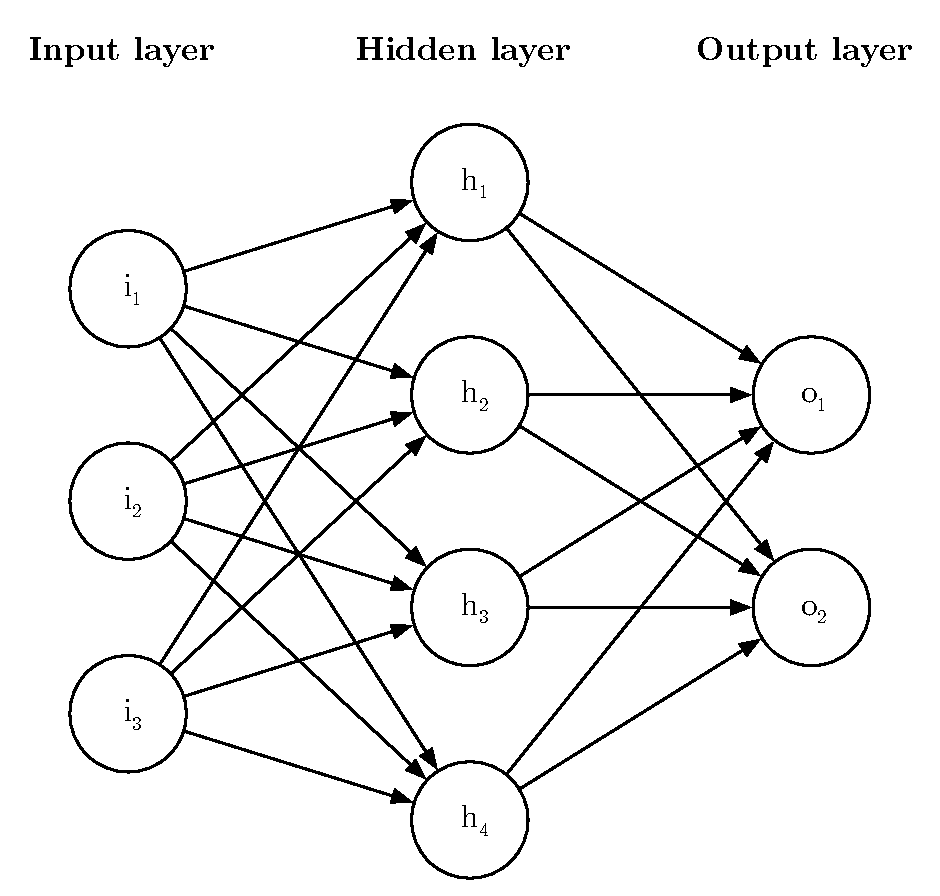
\includegraphics[width=0.6\linewidth]{fig/neural_network.eps}
	\caption{A neural network with one input layer composed of three neurons,
	one hidden layer of 4 neurons, and one output layer with 2 neurons.}
	\label{fig:neural_network}
\end{figure}


\section{Recurrent neural networks}
In some cases, it is a good idea to add a feedback loop to a neural network. 
A feedback loop such as the one shown in Figure~\ref{fig:rnn}, also called
a recurrent connection, poses evident issues for the backpropagation algorithm
since the depth of the neural network can become theoretically infinite.\\

A common way of training recurrent neural networks is to unroll them for a 
given, finite amount of time steps. The error signal can then be computed
for the output value at each time step, and backpropagated through all the
previous input values that affected its computing.\\

Recurrent neural networks are very useful in the context of reinforcement 
learning because they lay the ground for the memory aspect needed to solve
some tasks.

\begin{figure}[]
	\centering
	\subfloat[][A recurrent connection]{\qquad
		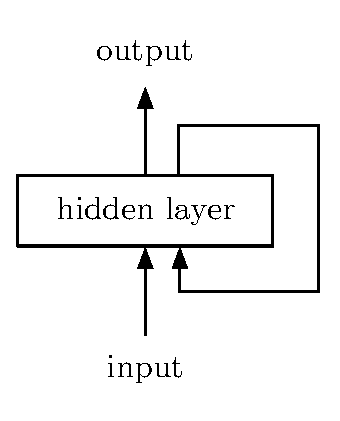
\includegraphics[width=0.1515\linewidth]{fig/recurrent_neural_network.eps}\qquad}
	\qquad
	\subfloat[][An unrolled recurrent neural network]{
		\includegraphics[width=0.6\linewidth]{fig/recurrent_neural_network_unrolled.eps}}
	\caption{Recurrent neural networks}
	\label{fig:rnn}
\end{figure}

\todo{universal function approximators}



\chapter{Reinforcement Learning}
\begin{quotation}
\noindent ``\emph{Tell me and I forget, teach me and I may remember, involve me
	and I learn.}''
\begin{flushright}\textbf{Benjamin Franklin}\end{flushright}
\end{quotation}

\vspace*{0.5cm}


\section{The reinforcement learning problem}
A reinforcement learning setting, as defined in Sutton and Barto \cite{suttonbarto}
sees two main components interact : the
\textbf{agent} (an entity performing actions) and the \textbf{environment}
(the world in which the agent is situated). 
The environment can be in several states which the agent
can observe. In some problems, the agent might not be able to observe the
full state of the environment (making the problem a partially observable one).  
The agent chooses actions based on its knowledge of the state of the
environment. These actions might (and often do) alter the state of the
environment, but will also generate a \textbf{reward}.  The
goal of the agent is to maximise the obtained reward.\\

With this simple setting, of which a diagram is shown in Figure~\ref{fig:rl},
we can design algorithms that can be trained to solve a huge variety of tasks
without ever having to include task-specific logic to the algorithm.\\

For example in the CartPole problem : the cart can be in several 
positions and have different velocities, and the pole has similar 
characteristics; the values of these characteristics constitute the state
of the environment. The agent has two actions at its disposal : nudge
the cart to the left, and nudge the cart to the right. 
The reward of the CartPole environment is +1 every timestep the pole is balanced
within a given angle 
and the cart is within a certain range on the rail, 0 otherwise.


\begin{figure}[]
	\centering
	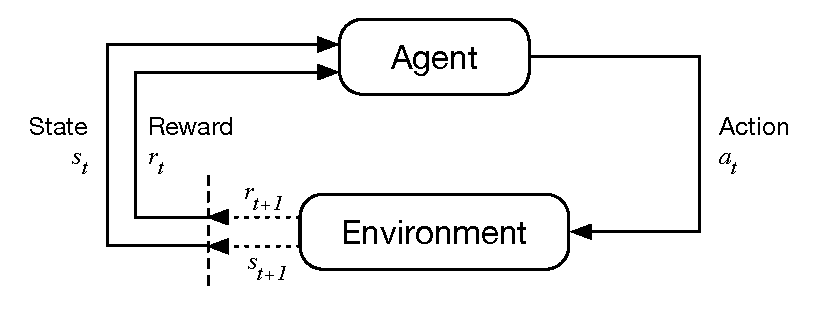
\includegraphics[width=0.65\linewidth]{fig/rl.eps}
	\caption{The setting of a reinforcement learning problem 
		\cite{suttonbarto}}
	\label{fig:rl}
\end{figure}

\subsection{Markov Decision Processes}
A reinforcement learning problem can be formally defined as a Markov 
Decision Process (MDP) \index{MDP} characterised by :
\begin{itemize}
	\item a set of states $\mathcal{S}$
	\item a set of actions $\mathcal{A}$
	\item a transition function 
		$T(s, a, s') = P(s_{t+1} = s' \mid s_t = s, a_t = a)$
	\item a reward function 
		$r(s, a, s') = \mathbb{E}
		 [r_{t+1} \mid s_t = s, a_t = a, s_{t+1} = s']$
\end{itemize}

The goal of reinforcement learning is for the agent to select, in any state it
can be in, the action that will lead it to the highest expected reward :

\begin{equation}
\label{eq:discounted_reward}
R_t = \mathbb{E}[r|\pi] = r_t + \gamma r_{t+1} + \gamma^2 r_{t+2}^2 + ... =
 \sum\limits_{i=0}^\infty \gamma^i r_{t+i}
\end{equation}

\noindent with $\pi$ the policy (see Section~\ref{sec:policy}) and 
the discount factor \index{discount factor} $\gamma \in [0, 1[$.
The discount factor allows one to tune the agent's behaviour on the
short-term/long-term spectrum. A discount factor $\gamma=0$ would mean that the
agent maximises its expected reward for the next transition only whereas a
discount factor close to one will favour behaviour that maximises long-term
reward, even if one action leads to a poor reward at first. It is chosen
by the designer as a hyperparameter for the whole length of the training.\\

\subsection{Policy}
\label{sec:policy}
\index{policy}
The agent uses a policy $\pi(a \mid s)$ to choose which action it is
going to play next. The policy describes a probability
distribution over the action set $\mathcal{A}$, determining the probability of
selecting each action $a_i \in \mathcal{A}$ once it is
in a certain state $s_i$.\\

We can call the policy \textbf{deterministic} if and only if:
\begin{equation}
\forall\, s \in \mathcal{S},\; \exists\, a \in \mathcal{A} : \pi(a \mid s) = 1
\end{equation}
\noindent In other words : in any state, only one action can be selected.
Otherwise, the policy is \textbf{stochastic}.

\section{An example : the 2-armed bandit problem}
\label{sec:rl_example}
The 2-armed bandit setting defines two actions that the agent can perform,
each of which associated with one arm. Each arm has an underlying reward
distribution -- for the sake of this example, let us define each arm with the
following Bernoulli distributions: \index{Bernoulli}

\begin{table}[H]
	\centering
	\begin{tabular}{c|c}
		Arm \#1 & Arm \#2 \\ \hline
		0.9 & 0.1
	\end{tabular}
\end{table}

\noindent This means that arm \#1 will generate a reward of 1 with a probability
of 0.9 and arm \#2 will generate a reward of 1 with a probability of 0.1.\\

The careful reader will have noticed that this problem is stateless 
($\mathcal{S} = \{\varnothing\}$), meaning that the agent only perceives
rewards and no state observations.\\

Of course, before its first interaction with the environment, the agent has no
information whatsoever about the reward distribution of each arm, and the whole
idea of reinforcement learning is to look for evermore efficient ways to learn
the structure and parameters of a problem in order to maximise reward.\\

One could imagine a simple strategy like the following : play each arm 10 times,
then always play the arm with the highest average reward. This policy is
deterministic, and yields either ($ \pi(a_1) = 1$ and $\pi(a_2) = 0$) or
($\pi(a_1) = 0$ and $\pi(a_2) = 1$). This could work in
our case, but might fail in cases where the distributions are much closer
(e.g. 0.45 and 0.55). What if the reward was sampled out of overlapping normal
distributions?\\

Deciding whether the following action should be used to explore the environment
and gain information about it; or to exploit the information already available
to try to maximise reward is not trivial. Exploring could make training slower
or affect the reward if our model of the environment is correct, but it is 
needed to increase the probability that we have indeed a correct model. This
tradeoff is called the exploration/exploitation tradeoff. \index{exploration}
\index{exploitation}\\

Sutton and Barto \cite{suttonbarto} propose two
simple ways to tackle this tradeoff : $\epsilon$-greedy and softmax selection.
Both methods fall within the denomination of Action-Value methods, meaning
that a value will be attributed to each action based on how well it did
in the past. Suppose action $a$ has been chosen $K_a$ times before timestep
$t$, and the agent has received rewards $r_1$, $r_2$,... while playing it. 
The value of action $a$ is:
\begin{equation}
Q_t(a) = \frac{r_1 + r_2 + ... + r_{K_a}}{K_a}
	\label{eq:action-value}
\end{equation}

\subsubsection{$\epsilon$-greedy}
This strategy keeps an average of the reward of each earm and chooses the next
action the following way:
\begin{equation}\begin{cases}
	\text{$a$ with $\max\limits_aQ_t(a)$} & \text{with probability } (1-\epsilon) 
	\\
	\text{random $a$} & \text{otherwise}
\end{cases}
\label{eq:egreedy}
\end{equation}
A high $\epsilon$ forces the agent to explore more, while a low $\epsilon$
allows for more exploitation of the agent's knowledge of the problem. 
$\epsilon$ is a hyperparameter of the agent, meaning that it will have to
be chosen by the designer depending on the problem and its parameters to 
strike an optimal balance between exploitation and exploration.

\subsubsection{Softmax selection}
Instead of selecting the best action with a given probability, the 
softmax selection method defines a distribution probability over the whole
action space $\mathcal{A}$. This is usually done by using a Boltzmann distribution
(also called a Gibbs distribution):
$$ \frac{e^{Q_t(a)/\tau}}{\sum_{i=1}^{n}e^{Q_t(i)/\tau}} $$
which defines the probability of selection for each action. $\tau$ is called
the \textit{temperature} parameter. A high temperature smooths the distribution,
making all actions more equally likely to be selected, and a low temperature
will tend to behave more like greedy action selection.

\section{Neural networks for reinforcement learning}
As hinted at previously, neural networks are powerful function approximators and
have yielded impressive results in reinforcement learning. They are used either
directly as policy functions, taking a state as input and outputting a
probability distribution over the action set; or as value estimators, by 
outputting a scalar which estimates the value of states and actions related to the
estimated achievable discounted reward from those states.

\subsection{Policy gradient methods}
Policy gradient methods are rather straightforward ways of learning to solve a task.
They assume that the policy is an end-to-end block of differentiable computation
(this could be a neural network, but other function approximators work too):
$$\pi(a \mid s)$$
This means that the policy $\pi$ takes as input the state, and outputs a 
probability distribution over the whole action set $\mathcal{A}$.\\

If we just received a good reward from the environment after choosing an action
$a$ from state $s$
with respect to the policy $\pi$, we could directly change the policy to 
increase the probability of selecting $a$ when we are in state $s$. The
experienced reader might have noticed that this process is very similar to
how we performed gradient descent to improve a classifier neural network in
the backpropagation section (\ref{sec:backprop}).
Indeed, classification is about increasing the probability of the correct
class when given a sample (or decreasing the probability of the wrongly
predicted class). Similarly to how class labels are backpropagated through
the differentiable function, we can backpropagate rewards.
Figure~\ref{fig:supervised_vs_pg} shows the process similarity between 
supervised learning and policy gradient methods.\\


\begin{figure}
	\centering
	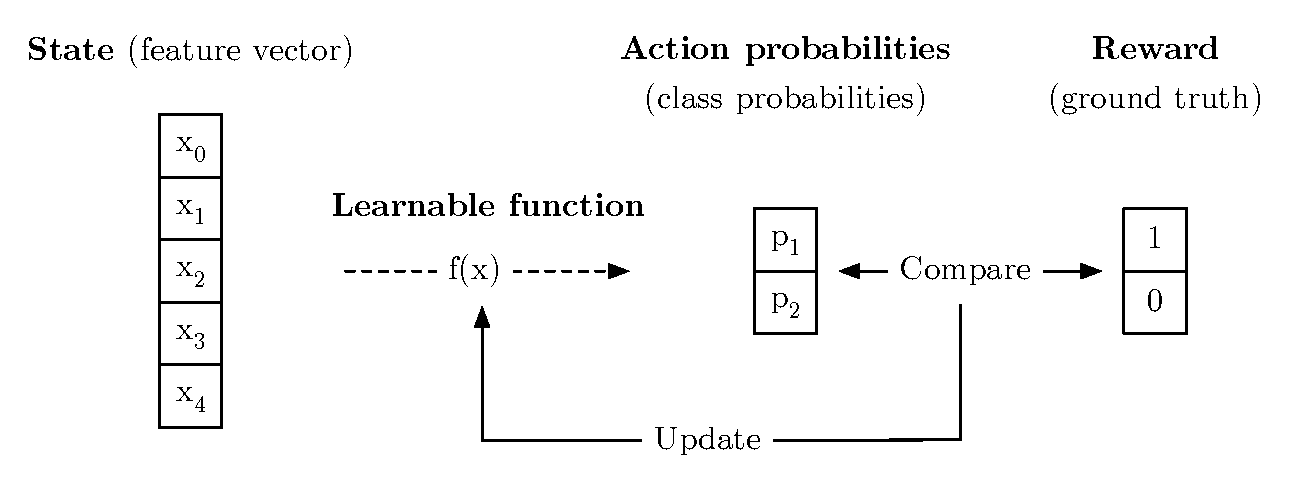
\includegraphics[width=0.8\linewidth]{fig/supervised_vs_pg.eps}
	\caption{The policy gradients process, and its similarity to
	the training process of supervised learning. Text in parentheses
	represents the supervised learning equivalent of the vectors 
	involved in policy gradients.}
	\label{fig:supervised_vs_pg}
\end{figure}

Let us assume that the
policy is defined by a neural network of which the input layer is set to 
receive an observation of the state of the environment and the output layer
defines a policy (a probability distribution over the actions set).
Training starts with a randomly initialised policy. 
When the agent performs an action chosen with its policy, the environment will
update its state and the agent will receive an observation of this state as
well as a reward signal. We can use the reward signal to proportionately
encourage (if the reward is 
positive) or discourage (if the reward is negative) taking this action in 
this specific state.\\

As the policy is defined by a neural network, we have to define a way to
update the network to find the best policy. This is done by defining a loss
function of which the gradient will be propagated back into the network, or
by defining directly the gradient as a parameters update rule.\\

Let us suppose that the agent is in an environment where it can perform two
actions, and it has received a reward of +5 after choosing action 2
sampled out of its policy $\pi(s) = [0.1, 0.9]$. We can directly use the
reward signal as a scaler for the gradient to update the network. Indeed,
multiplying the gradient of the policy $\nabla \pi(a \mid s)$ by 
$[0, 5]$ (because a +5 reward was generated by action 2) will make the network
learn which actions to perform under certain states by directly increasing the
probability of playing actions which receive a positive reward, and by
decreasing the probability of actions which receive a negative reward.\\

We can prove mathematically that multiplying the gradient of the policy
equates to the gradient of the expected reward from state $x$:
\begin{align*}
	\nabla \mathbb{E}_x[r(x)] &= \nabla \sum\limits_x\pi(x)r(x)\\
	&=  \sum\limits_x \nabla\pi(x)r(x)\\
	&=  \sum\limits_x \pi(x)\frac{\nabla\pi(x)}{\pi(x)}r(x)\\
	&=  \sum\limits_x \pi(x)\nabla\log(\pi(x))r(x)\\
	&=  \mathbb{E}_x[r(x)\nabla\log(\pi(x))]\\
\end{align*}

The method as presented still presents an issue in the sense that it only takes
into account immediate reward, and we may want to maximise long-term reward.
Let $R_t$, the discounted future reward at time step $t$ (see equation 
\ref{eq:discounted_reward}), be the metric
that we want to maximise. In a policy gradients method, we will update the
neural network policy directly with :
\begin{equation}
	\label{eq:policy_update_rule}
	\alpha \nabla \pi(a \mid s) R_t
\end{equation}
in which $\alpha$ is the learning rate and $a$ was the chosen action.

\subsection{Value methods}
There is another category of methods which use an estimate of the value of
actions or states; in other words functions which map states or state-action
pairs to estimates of their discounted future reward $R_t$. We have seen
examples of such functions previously: $\epsilon$-greedy and softmax
selection both are value-based methods (see Section~\ref{sec:rl_example} and
more specifically equation~\ref{eq:action-value}).\\

There is an important
difference between value-based methods and policy gradient methods: in the
former, the policy has to be defined by hand whereas the latter are
end-to-end (meaning that the policy is learned too). In value-based methods,
the model designer has to choose a policy that selects an action based
on estimations provided by value functions.\\

\subsubsection{V-values} 
Let us consider a problem with a relatively small set of states 
$\{s_1, s_2, ..., s_k\}$. We could estimate the \textbf{value} of 
states based on the expected discounted reward we can reach from each state, 
based on a policy $\pi$: 
$$ V^\pi(s) = R_t = \mathbb{E}
   \left[ r_t + \gamma r_{t+1} + \gamma^2 r_{t+2}^2 + ...  \right]$$
At first however, this estimate is not known. Let us imagine a problem where
only one state $s_o$ generates a reward of +100, and a state $s_{o-1}$ is a state
adjacent to $s_o$. We choose to use a discount factor $\gamma = 0.9$. 
Whenever the agent plays the action that makes it go from
$s_{o-1}$ to $s_o$, the agent receives a reward of +100. Its value for $s_o$ is:
$$V^\pi(s_o) = r_t = 100$$
What about the value of $s_{o-1}$? Being right next to the goal state, it should
have quite a high value, while at the same time being lower than the goal state.
This is exactly what happens if we use our value estimation formula:
$$V^\pi(s_{o-1}) = r_t + \gamma r_{t+1} = 0+ 0.9 \times 100 = 90$$
What about a state $s_{o-2}$ adjacent to $s_{o-1}$ but not $s_{o}$? We would
compute:
$$V^\pi(s_{o-2}) = r_t + \gamma r_{t+1} + \gamma^2 r_{t+2} = 0+ 0 + 0.9^2 \times 100 = 81$$

The reader might have noticed that there is a simpler way to estimate values
than by unrolling the agent's full experience until it gets a reward. 
We can indeed use a Bellman equation to rewrite our estimation using
the values of adjacent states only by iterating on our current estimates:
\begin{equation}
V_{k+1}^\pi(s) = R_t = \mathbb{E}
   \left[ r_t + \gamma r_{t+1} + \gamma^2 r_{t+2}^2 + ...  \right] = 
   \mathbb{E}\left[ r_t + \gamma V_k^\pi(s')\right]
\label{eq:vupdate}
\end{equation}
where $s'$ is the state of highest value that can be reached from $s$ and $k$
is the iteration number. We could rewrite this equation as the following:
$$ V_{k+1}^\pi(s) = \max\limits_a \sum\limits_{s'} p(s\mid s,a)\left[r(s,a,s') + 
\gamma V_{k+1}\pi(s')\right]$$

Iterating over estimates means that we start off with a nonoptimal value
function. It would theoretically take an infinite amount of iterations to
converge to an optimal value function $V^*(s)$, but we generally stop once the
value function changes by a small enough amount.\\

Once again, we can
use neural networks to estimate such functions. We then only have to define
a policy that decides which actions to take given these value estimates; one
example of such a policy could be a deterministic policy choosing the action
leading to the state with the highest value.\\

Equation \ref{eq:vupdate} can be used as an update rule for the $V^\pi$ network 
parametrised by its weights $\theta$ with a loss similar to :
\begin{equation}
	\label{eq:v_update_rule}
	\left[V^\pi(s\mid \theta_t) -  \left(r_t + \gamma V^\pi(s'\mid \theta_{t-1}) \right)\right]^2 
\end{equation}
\noindent which is a simple mean squared error between the estimation $V^\pi(s\mid \theta_t)$ and
the target $\left(r_t + \gamma V^\pi(s'\mid \theta{t-1}) \right)$.

\subsubsection{Q-values} 
Q-values estimate the value of state-action pairs instead of
only states; i.e. the
estimated discounted reward achievable when taking a specific action in a 
specific state. The reasoning to find an update rule is similar for V-values
and Q-values. The optimal Q function can be estimated with a Bellman equation :
$$ Q(s, a) = \mathbb{E}\left[ r_t + \gamma \max\limits_{a'} Q(s', a') \right]$$
\noindent and so can be deduced an update rule for Q networks of which the loss
can be defined with the following :

\begin{equation}
	\label{eq:q_update_rule}
\left[Q(s, a\mid \theta_t) - 
	\left( r_t + \gamma \max\limits_{a'} Q(s', a'\mid \theta_{t-1}) \right) \right]^2
\end{equation}

\subsubsection{Value networks in real life : DQN}
Estimating values using neural networks has an enormous advantage over using
tables of values. Using tables becomes intractable as the size of the state
space increases (or action space in the context of Q-values); worse, they become
unusable if the state space becomes continuous, unless we discretise it,
which might cause unwanted artifacts.\\

However, neural networks are not always stable, and they couldn't be used
for complex reinforcement learning tasks until Mnih et al \cite{dqn, dqn_nature}
proposed their Deep Q-network architecture. In their setting, Mnih et al. 
use the loss function described in equation \ref{eq:q_update_rule} with two
key modifications that allow the network to learn in a stable way:

\paragraph{Replay memory} Instead of updating the network using only the 
last transition that the agent went through (the tuple $(s, a, r, s')$), 
Mnih et al. sample a transition from a replay memory in which are stored
a large number of played transitions. This allows the agent to decorrelate
samples that come from the same sequence of transitions.

\paragraph{Target network} Equation \ref{eq:q_update_rule} uses a Q-value
estimate from the previous timestep as a target. This can cause oscillation
and divergence. To mitigate these effects, Mnih et al. proposed using a target
network in which the weights are copied from the network being trained 
only periodically.\\

Another key component of Mnih et al.'s architecture is the use of
convolutional neural networks \cite{convnets} which take advantage of the
relevance of spatial context in an image state. We won't delve into the
description of such networks as they won't be needed in this work.

\subsection{Actor-Critic}
We can call policy gradient methods "actor-only" methods as the methods
only choose actions without evaluating them \textit{per se}. On the other
hand, value-based methods can be called "critic-only" methods as they
evaluate possible actions and states but do not provide the agent
with a choice of action.\\

There is a third category of methods which mixes both approaches. 
Actor-critic methods \cite{suttonbarto} have both an \textit{actor} (the policy) and a
\textit{critic} (value functions). The actor performs the actions, and the 
critic updates the policy. One way to update the policy using a critic is to
scale the policy gradient using our current estimate of the V function:
\begin{equation}
	\label{eq:adv_update_rule}
\nabla \pi(a_t \mid s_t) (R_t - V(s_t))
\end{equation}
This way, the policy will be updated according to how wrong the critic was.
The value $R_t - V(s_t)$ is called the \textbf{advantage} \index{advantage}
because it expresses how much better (or worse) the reward was compared to 
what was estimated \cite{advantage, a3c}.


\subsubsection{The A2C algorithm}
We now have all the cards in our hand to understand the A2C
(Advantage Actor-Critic) algorithm which is a simpler version of A3C \cite{a3c}
(it only uses one thread instead of being asynchronous). 
A2C consists of a neural network
of which the input is the state $s_t$, and which outputs both a value function
$V(s_t)$ and a policy $\pi(s_t)$ (see Figure~\ref{fig:a2c}). These outputs
respectively use the update rules described in equations \ref{eq:v_update_rule}
and \ref{eq:adv_update_rule}. The first loss function computes the error
related to the policy output:
$$ \mathcal{L}_p = \pi(a_t \mid s_t) (R_t - V(s_t))$$
and the second loss computes the error related to the value output
$$ \mathcal{L}_v = (R_{t-1} - V(s_t))^2$$
The complete loss function for the A2C agent is:
$$ \mathcal{L} = \beta_v \mathcal{L}_v + \beta_p \mathcal{L}_p $$
where $\beta_v$ and $\beta_p$ are hyperparameters used to scale both losses.\\

Algorithm~\ref{algo:a2c} shows the training
process of the A2C agent which alternates playing episodes and updating the
network according to the agent's experience.

\begin{figure}[]
	\centering
	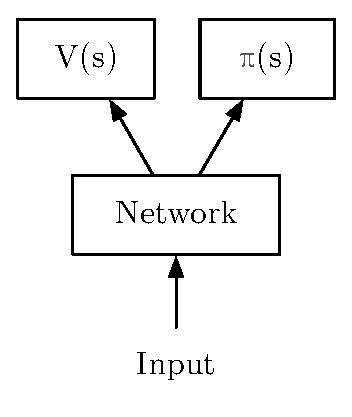
\includegraphics[width=0.2\linewidth]{fig/a3c.eps}
	\caption{The A2C network}
	\label{fig:a2c}
\end{figure}

\begin{algorithm}
\caption{The A2C training process}
\label{algo:a2c}
\begin{algorithmic}[1]
\State{$T_{\text{max}} \leftarrow$ maximum number of ticks}
\While{$T < T_{\text{max}}$}
	\Statex
	\State{\textit{// Play an episode}}
	\State{$t \leftarrow 0$}
	\While{$t <$ maximum episode length \textbf{and} episode not finished}
		\State{perform $a_t$ sampled using $\pi(s_t)$}
		\State{record reward $r_t$ and new state $s_{t+1}$}
		\State{$t \leftarrow t+1$}
	\EndWhile
	\State{$T \leftarrow T + t$}
	\Statex
	\State{\textit{// Compute advantages and gradients by unrolling episode}}
	\State{$d\theta_p \leftarrow 0$ \textit{// policy gradient}}
	\State{$d\theta_v \leftarrow 0$ \textit{// value gradient}}
	\For{$i \in \{t-1,\; t-2,\; ...,\; 0\}$}
		\State{$R \leftarrow r_i + \gamma R$}
		\State{$d\theta_p \leftarrow d\theta_p + \nabla \pi(a_i|s_i)(R-V(s_i))$}
		\State{$d\theta_v \leftarrow d\theta_v + \nabla (R - V(s_i))^2$}
	\EndFor
	\State{Update policy network using $d\theta_p$}
	\State{Update value network using $d\theta_v$}
	\Statex
\EndWhile

\end{algorithmic}
\end{algorithm}

\subsubsection{Summary}
Reinforcement learning is the study of the behaviour of an agent situated in
an environment generating rewards for the agent. Many existing techniques
allow the agent to learn to perform well in many environments, and 
using neural networks to solve reinforcement learning problems has shown
to be very powerful.\\

We will now see how we can adapt the A2C agent to perform meta reinforcement
learning.




\part{Meta Reinforcement Learning}
\chapter{Learning to learn}
\begin{quotation}
\noindent ``\emph{All of the biggest technological inventions created by man -
	the airplane, the automobile, the computer - says little about his 
	intelligence, but speaks volumes about his laziness.  }''
\begin{flushright}\textbf{Mark Kennedy}\end{flushright}
\end{quotation}

\vspace*{0.5cm}

\section{Goals and foundations}
Developing and tuning algorithms to find the optimal strategy to solve a
reinforcement learning problem is hard. Some of the challenges one meets are:
\begin{itemize}
	\item the tradeoff between exploration and exploitation
	\item designing a strategy that allows for versatile training
	\item choosing hyperparameters (learning rate, architecture of a
		neural network,...) \index{hyperparameter} that make the strategy
		optimal considering the reinforcement learning problem at hand.
\end{itemize}

Let us consider the problem of learning a simple bandit problem with dependent
arms. Say, for example, that a bandit has two arms, each of which producing
a reward according to a Bernoulli distribution with the following parameters :
$$ \begin{cases} P(r \mid \text{arm}_1) = p_b \\ 
P(r \mid \text{arm}_2) = 1 - p_b  \end{cases} $$
where $P(r \mid \text{arm}_1)$ is the probability of arm 1 to generate a reward
and $0 \leq p_b \leq 1$ is the parameter of the bandit problem. One way to
solve this problem would be to use the $\epsilon$-greedy strategy (see
Section~\ref{sec:rl_example}). \\

This raises the question about choosing $\epsilon$. Choosing a low $\epsilon$
encourages exploitation but we have a higher chance of wrongly estimating $p_b$.
Choosing a high $\epsilon$ doesn't allow the agent to perform optimally once
its knowledge about the parameters of the problem is likely to be optimal.
Moreover, we could choose a variable $\epsilon$, high at first but slowly
converging to 0, but we then are faced with the choice of another
hyperparameter: the number of steps over which $\epsilon$ should be annealed.\\

One could propose using a more advanced method, and there are many. Multi-armed
bandits have been heavily studied and to this day, several algorithms exist to
solve the kind of bandit problems defined above very quickly - i.e. to explore
just enough to implicitly learn $p_b$ so to exploit the best arm as much as
possible. Examples of these algorithms are the Gittins indices algorithm
\cite{Gittins79banditprocesses},
UCB \cite{Auer:2002:FAM:599614.599677} and Thompson sampling
\cite{thompson1933}.\\

The obvious problem here is that we can always choose to manually design more
and more sophisticated techniques and to tune more perfectly their parameters,
but could we not instead use reinforcement learning to do this for us instead?\\

Recently, Wang et al. \cite{learningtorl} and Duan et al. \cite{fastrlviaslowrl}
proposed the idea of using reinforcement learning to learn an algorithm which
deploys an optimal strategy for a class of problems sharing a similar structure.
We will use the name "meta-RL" or meta-learning for this technique, as proposed 
by Wang et al. \\
\begin{figure}
	\centering
	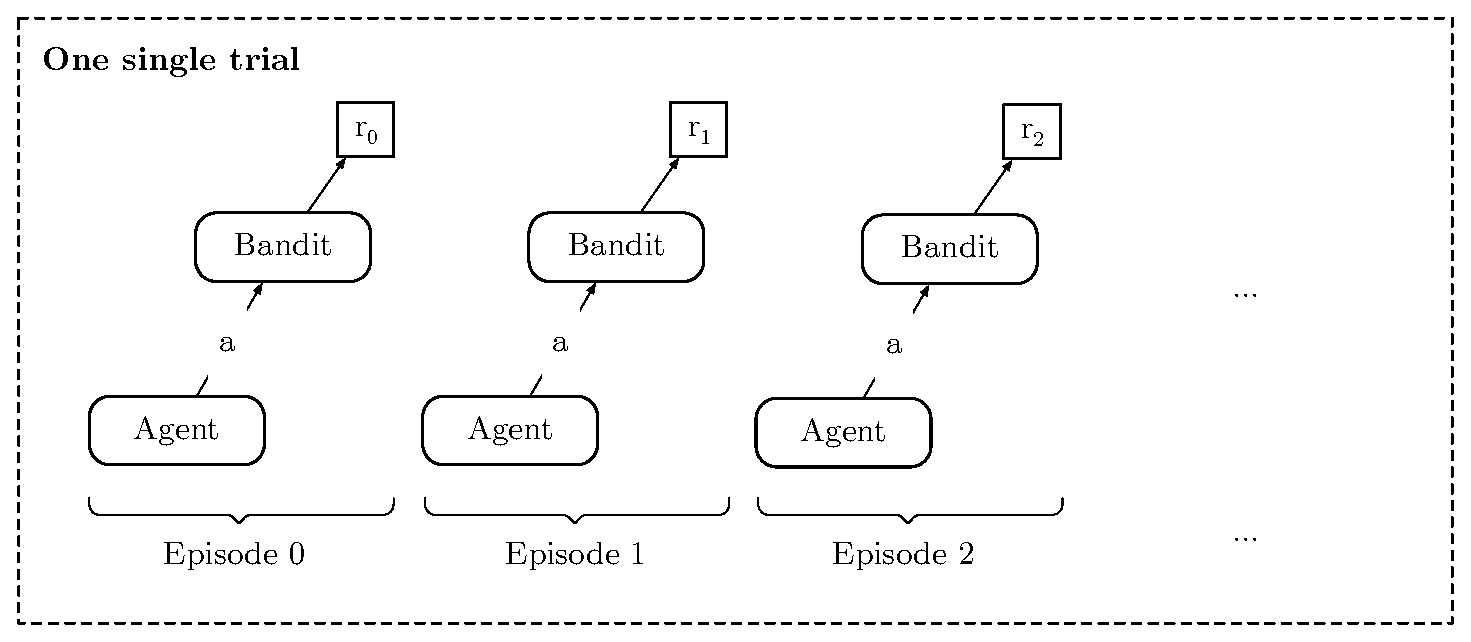
\includegraphics[width=0.7\linewidth]{fig/normal_bandit_training.eps}
	\caption{A classic training sequence to learn a bandit problem. One
	manually designs a strategy which inspects the reward obtained at 
	the end of an episode and evaluates accordingly the performance of the action
	taken. The strategy then updates the policy inbetween episodes.}
	\label{fig:normal_bandit_training}
\end{figure}

In classic reinforcement learning (see Figure~\ref{fig:normal_bandit_training}),
\textbf{the network represents a policy.} Its goal is to maximise its reward
for each episode, and it is trained by looping the following steps:
\begin{enumerate}
	\item let the network play an episode
	\item update the network using a hand-designed strategy (Gittins, UCB,
		Q-learning \cite{qlearning}, SARSA \cite{sarsa}, ...) to 
		increase the total reward of an episode
\end{enumerate}

As stated at the beginning of this chapter, designing strategies to learn
policies is a hard task and can demand a sensitive tuning of parameters.
In meta-RL, \textbf{the network represents an algorithm which learns a policy}
Its goal is to be the best possible learning strategy, which is why we train
it differently:
\begin{enumerate}
	\item let the network play a \textbf{trial} \index{trial} of several
		episodes of the same problem
	\item update the network so that it learns faster
\end{enumerate}
In this context, the network has to maximise its expected reward across
\textbf{all} episodes of a trial (see 
Figure~\ref{fig:meta_bandit_training}). Note that a trial replicates the setting
of learning to solve a problem -- the agent is not learning to solve a 
problem anymore, it is learning to learn how to solve a problem, but in 
a very low number of episodes rather than the many episodes needed 
to train a standard reinforcement learning agent. This will incentivize the agent
to understand the structure of a problem and develop a strategy that allows it 
to estimate the parameters of the problem as fast as possible.
Generally, we will call the learned policy the inner 
algorithm, and the algorithm that learns the policy the outer algorithm.\\


\begin{figure}
	\centering
	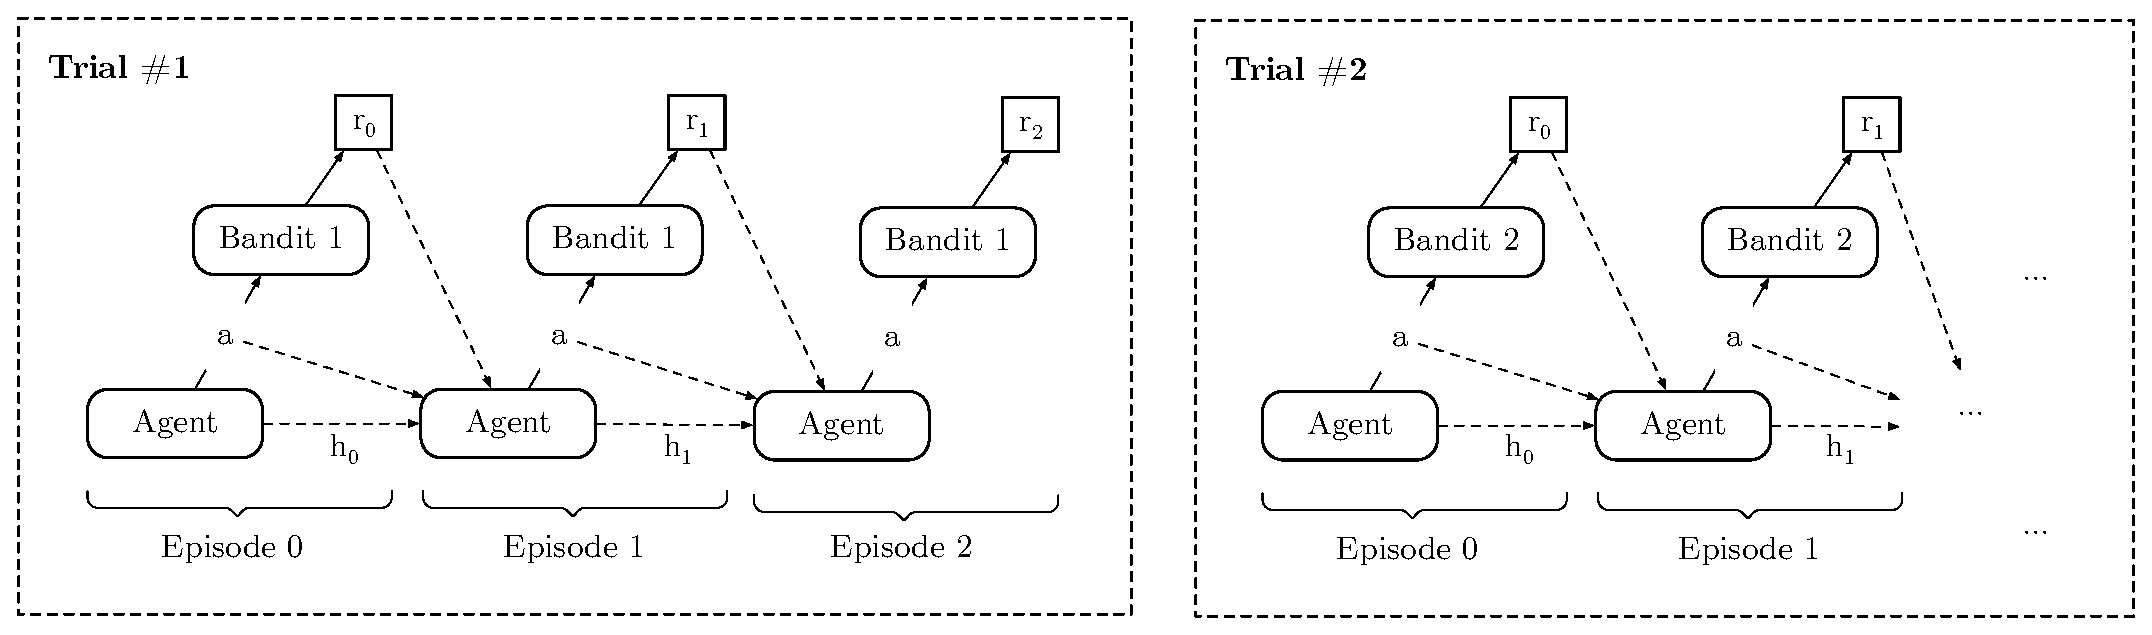
\includegraphics[width=\linewidth]{fig/meta_bandit_training.eps}
	\caption{The training sequence for a meta-RL agent on a bandit problem.
	In this case, the agent is left to play several episodes on its own
	without changing its weights. It is only when a trial ends that the
	outer algorithm evaluates the rewards of all episodes in the trial and
	updates the weights of the inner algorithm so that it increases its
	chances of having a better reward across all episodes. For trials of 
	three episodes such as the one presented in this figure, the outer
	algorithm forces the inner algorithm to learn the problem in 
	three episodes.}
	\label{fig:meta_bandit_training}
\end{figure}

In our manually designed strategies, we use previous actions and rewards
to update the policy and make it better. Similarly, in order to
make meta-RL work, the agent has to receive as input the previous reward
and the action that led to that reward, but it also needs to carry on some
sort of memory of past actions and rewards. We do this manually in 
$\epsilon$-greedy by keeping track of the average reward yielded by each arm.
In the case of meta-RL, this is done by using a recurrent network which
carries a hidden state from the first episode in the trial to the last.\\


\begin{figure}
	\centering
	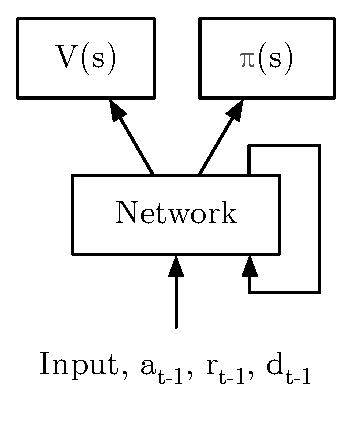
\includegraphics[width=0.2\linewidth]{fig/a2c_meta.eps}
	\caption{The meta-learning A2C agent. The key difference with a
	standard A2C agent is that it receives the values 
	$[a_{t-1},r_{t-1},d_{t-1}]$ in addition to the state observation. It
	is of course also trained in a different way to a standard A2C agent.}
	\label{fig:a2c_meta}
\end{figure}



The general setup presented by Wang et al. uses a recurrent neural network of
which the weights, once trained "slowly" over several trials of multiple
episodes, will encode the "fast" learning policy.
Figure \ref{fig:a2c_meta} shows the meta-learning A2C agent presented in Wang
et al. \cite{learningtorl}. There are two differences to note compared to
Figure~\ref{fig:a2c}: the first one is the recurrent connection, and the
second one is the set of values we input to the agent at each time step. In
addition to the state of the environment, we add the previous action, 
previous reward and a termination flag which is set to 1 when an episode
has reached a terminal state; 0 otherwise.\\

\begin{figure}[H]
	\centering
	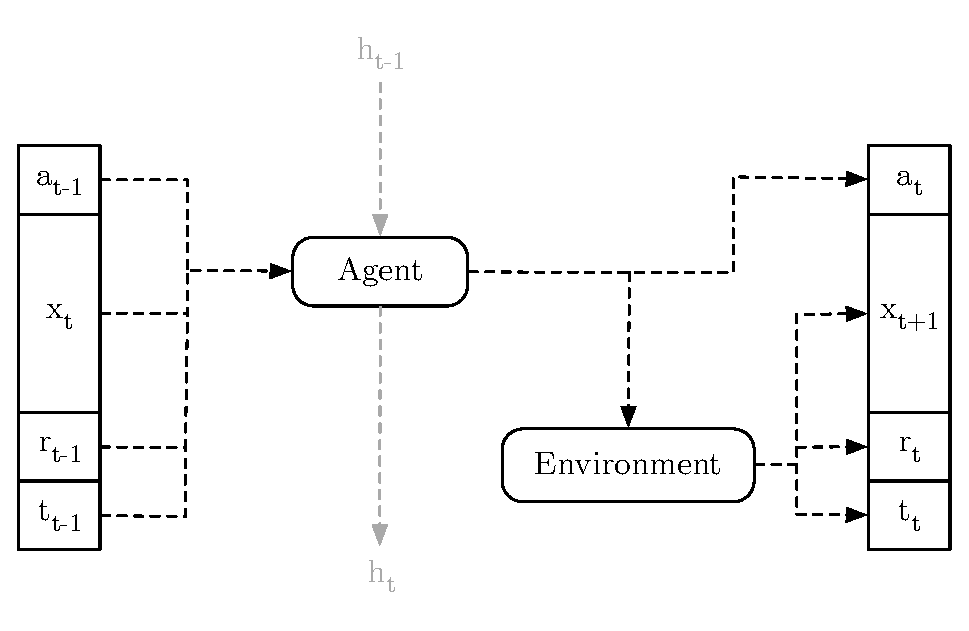
\includegraphics[width=0.6\linewidth]{fig/meta_rl_timestep.eps}
	\caption{An unrolled timestep in the meta-RL training setting. At each
	timestep, the agent receives an observation of the state of the
	environment as well as the previous action taken, the associated reward,
	and the termination flag. It also receives its previous hidden state
	if and only if the previous timestep was part of the same trial (this
	could still mean that the last timestep was from a different episode
	which just terminated)}
	\label{fig:meta_rl_timestep}
\end{figure}


It is important to emphasize on the fact that the agent passes on its hidden
state between different episodes of the same trial (and if episodes last for
more than one timestep, between timesteps as well), but \textbf{not} between
trials (see Figure~\ref{fig:meta_bandit_training}).
The reason why the inter-episode connection is needed is because
the agent might want to deploy a different policy given the results of 
previous episodes as it has to optimise its expected reward across multiple
episodes.

\section{Agent architecture}
\begin{figure}
	\centering
	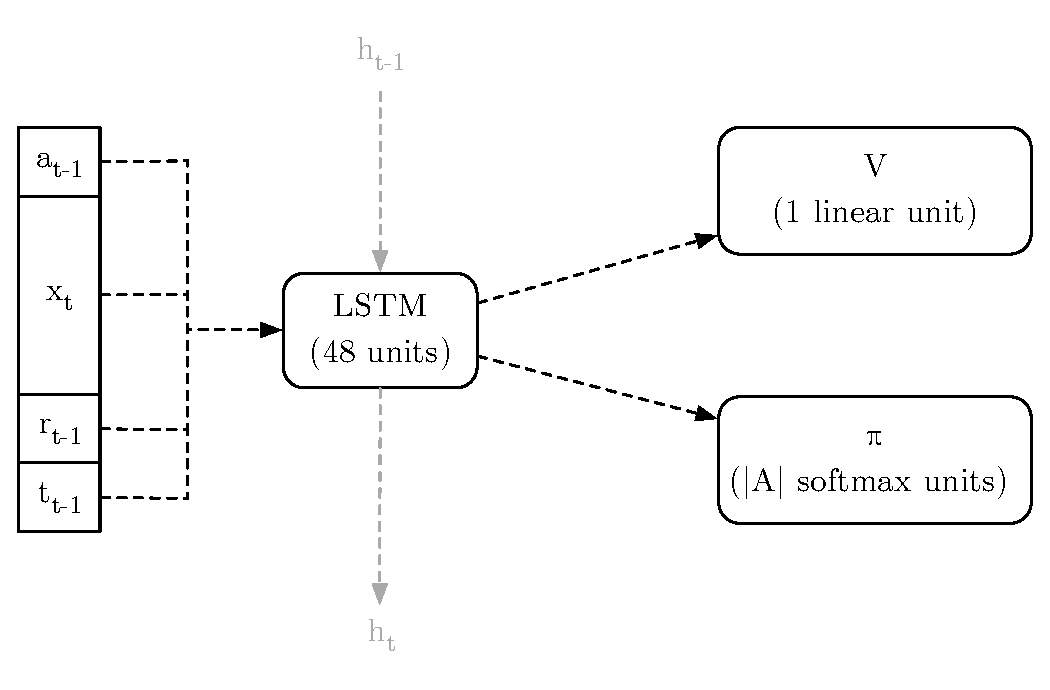
\includegraphics[width=0.7\linewidth]{fig/agent_architecture.eps}
	\caption{Architecture of the meta-learning A2C agent}
	\label{fig:agent_architecture}
\end{figure}
We use the same A2C agent that Wang et al. \cite{learningtorl} have used
for their bandit experiments. It is described in Figure~\ref{fig:agent_architecture}.
The input vector is a concatenation of the state observation, the previous
action taken, the reward obtained at the previous timestep and the termination
flag :
$$ i = [s_t, a_{t-1}, r_{t-1}, d_{t-1}] $$
The action taken is converted to a one-hot encoding (converting the action
index into a vector of length $|\mathcal{A}|$ containing zeros except a single
1 at the index of the action). This vector is then fed to a LSTM sized at 48
hidden units, followed by two branches :
\begin{enumerate}
	\item a fully connected softmax layer with $|\mathcal{A}|$ units (the policy
		output). Actions are selected by sampling according to the
		distribution defined by the policy, rather than by taking the
		action with the highest probability.
	\item a fully connected linear layer with 1 unit (the value output).
\end{enumerate}
The loss of the A2C agent is the following : 
$$ \mathcal{L} = \beta_v \mathcal{L}_v + \beta_p \mathcal{L}_p - \beta_e 
 \mathcal{L}_e $$
where $\mathcal{L}_v$ is the value loss : 
$$ \mathcal{L}_v = (R_{t-1} - V(s_t))^2$$
$\mathcal{L}_p$ is the policy loss : 
$$ \mathcal{L}_p = \pi(a_t \mid s_t) (R_t - V(s_t))$$
$\mathcal{L}_e$ is the entropy regularisation : 
$$ \mathcal{L}_e = \sum\limits_{a \in A}\pi(a \mid s_t)\log(\pi(a \mid s_t))$$
and $\beta_v = 0.5$, $\beta_p = 1$, $\beta_e = 0.05$. An update is performed
once after every trial using Adam \cite{adam} with a learning rate of 0.001.\\

Unless stated, the discount factor used in all experiments is $\gamma=0.9$. 


\section{Meta-learning dependent bandits}
Let us come back to the problem stated previously as an example. This will
prove useful as it is the same setting used by Wang et al. \cite{learningtorl}.
We can then compare our results with theirs to introduce the current state
of the art, test our implementation and verify that their results can 
be reproduced. This setting has the advantage of being relatively simple
so it will help us understand meta-learning before jumping to a harder problem.\\

The setting is the following: a dependent
bandit with 2 arms of which the reward distribution is a Bernoulli distribution
with the following parameters : 
$$ \begin{cases} P(r \mid \text{arm}_1) = p_b \\ 
P(r \mid \text{arm}_2) = 1 - p_b  \end{cases} $$

We define a training distribution of dependent problems with
$p_b \in [0.1, 0.2, 0.8, 0.9]$, creating the following set of dependent
bandit problems:
\begin{table}[H]
	\centering
	\begin{tabular}{c|c}
		Arm \#1 & Arm \#2 \\ \hline
		0.1 & 0.9 \\ \hline
		0.2 & 0.8 \\ \hline
		0.8 & 0.2 \\ \hline
		0.9 & 0.1
	\end{tabular}
\end{table}

The agent will play trials of 100 episodes - meaning that we choose one bandit
problem and let the agent pull either one of its arms 100 times, then reset
the hidden state and start again. Since the problem is stateless, the agent
only receives the last action taken, the previous reward and the termination
flag as input. The discount factor $\gamma$ is set to 0.8 to replicate 
Wang et al.'s experiment \cite{learningtorl}.\\

Wang et al. \cite{learningtorl} achieved creating a meta-learning
agent that could learn a dependent problem as the one defined above in only 
a few episodes (one episode being one pull of the bandit). For some experiments,
their agent outperforms the state of the art; and a look over the behaviour
of their agent shows only a minimal number of episodes spent exploring before
exploiting only.\\

Figure~\ref{fig:bandit_reward} shows that after some time, the agent figures out
a way to yield an excellent reward over all trials: for trials using bandits
with $p_b \in [0.2, 0.8]$, even if the agent pulled the best arm for
each episode (which rules out exploration completely), the total reward
expectation is 80, and for trials using bandits with $p_b \in [0.1, 0.9]$, 
the total reward expectation is 90. Scoring an average trial reward between
80 and 85 looks very close to optimal, if not fully optimal.\\

\begin{figure}[H]
	\centering
	\includegraphics[width=0.75\linewidth]{fig/bandit_reward.pdf}
	\caption{Evolution of the smoothed reward of trials during training on
	dependent bandit problems}
	\label{fig:bandit_reward}
\end{figure}

If we look at the evolution of decisions taken by the agent during training
on Figure~\ref{fig:bandit_optimality}, and especially on
Figure~\ref{fig:bandit_optimality}b, we see that the agent evolves from playing
randomly each arm to testing both arms for just a few episodes at the start
of the trial to then always play what it judges is the best episode.\\

\begin{figure}[H]
	\centering
	\subfloat[][Pulled arm]{
		\includegraphics[width=0.49\linewidth]{fig/bandit_pulls.png}}
	\subfloat[][Optimality of the pulled arm]{
		\includegraphics[width=0.49\linewidth]{fig/bandit_optimality.png}}
	\caption{Insight into the evolution of which arms get pulled and 
	whether they are optimal during training. On the left, a black dot
	represents the fact that arm \#1 has been pulled and a white dot
	represents the fact that arm \#2 has been pulled. On the right, a white
	dot signifies that the best arm has been pulled. This figure shows
	that after a bit of training, the agent learns to quickly identify
	which arm is the optimal arm and pulls that arm only after only 
	a few episodes.}
	\label{fig:bandit_optimality}
\end{figure}

We should emphasize on the importance of these results. If we had used the 
$\epsilon$-greedy method as is, the difference in performance would be 
significant on several aspects:
\begin{itemize}
	\item with a fixed $\epsilon$, sticking to the optimal arm would have
		been impossible (as a random action is required from time to 
		time), hindering performance while it can be very clear
		which arm is the best
	\item even if we chose a small $\epsilon$ to minimise performance loss
		in the exploitation phase, we would have increased dramatically
		the probability of not exploring enough at the start of the 
		episode
	\item similar reasoning can be used to argue about the number of 
		trials over which $\epsilon$ could have been annealed from
		1 to 0.
\end{itemize}
Using meta-learning allowed us to bypass all these design considerations.
Furthermore, both Wang et al. \cite{learningtorl} and Duan et al. 
\cite{fastrlviaslowrl} show that the strategy deployed by the meta-learning
agent matches (or outperforms) the best hand-designed strategies such as 
UCB and Gittins.\\

It is worth noting however that we have only been considering known and seen
bandit problems in our discussion so far. Nevertheless, we see 
on Figure~\ref{fig:bandit_test} that the meta-learning agent can generalise to
all other values of the parameter $p_b$ with very good performance. For the 
performance analyis of Figure~\ref{fig:bandit_test}, we let the agent play 
100 trials of 20 equally spaced values of $p_b$ in the range $[0.5, 0.975]$.
For each trial, the optimal arm was randomly shuffled to be either the first
or second arm. We compare the average reward obtained to the optimal expected
reward (the theoretical expected reward obtained by exclusively pulling the
optimal arm, which is not practically possible since the agent doesn't know
which arm is the optimal arm and has to explore for several episodes).\\

The agent performs very well on unseen values of $p_b$, even harder ones which
are closer to 0.5, even though it has only ever seen $p_b = 0.8$ and $p_b = 0.9$.

\begin{figure}[H]
	\centering
	\includegraphics[width=0.8\linewidth]{fig/bandit_test.pdf}
	\caption{Average performance of the meta-learning agent on the whole
	range of the parameter $p_b$. The agent has only seen
	$p_b \in [0.8, 0.9]$. The performance is compared to the theoretical
	expected reward if the agent selected the optimal arm for each episode.}
	\label{fig:bandit_test}
\end{figure}


\subsubsection{Summary}
Now that we have laid out the stakes and goals of meta reinforcement learning,
explained the training process and the architecture of the agent,
and recreated state of the art experiments to verify both our implementation
and the results obtained in the literature; we will extend the application
of meta learning to a new class of problem. We will derivate a distribution
of tasks from the CartPole problem and analyse the performance and dynamics
of meta-learning applied to this case.



\chapter{Knowledge gain with multiple episodes}
\begin{quotation}
\noindent ``\emph{quote}''
\begin{flushright}\textbf{author}\end{flushright}
\end{quotation}

We will first and foremost analyse how a reinforcement learning agent 
performs when it is confronted to playing a single episode of one of the 
CartPole problems. We will train the agent on a distribution of 20 permutations
(shown on Table~\ref{tab:20perms}), at first without inverting the agent's
action.

\begin{table}
	\centering
	\caption{State permutations used for training and testing}
	\label{tab:20perms}
	\subfloat[Training distribution]{
		\bgroup
		\def\arraystretch{1.5}
		\begin{tabular}{c|c|c}
			[0, 1, 2, 3] & [1, 0, 2, 3] & [2, 0, 1, 3] \\
			\hline
			[0, 1, 3, 2] & [1, 0, 3, 2] & [2, 0, 3, 1] \\
			\hline
			[0, 2, 1, 3] & [1, 2, 0, 3] & [2, 1, 0, 3] \\
			\hline
			[0, 2, 3, 1] & [1, 2, 3, 0] & [3, 0, 1, 2] \\
			\hline
			[0, 3, 1, 2] & [1, 3, 0, 2] & [3, 0, 2, 1] \\
			\hline
			[0, 3, 2, 1] & [1, 3, 2, 0] & [3, 1, 0, 2] 
		\end{tabular}
		\egroup
	}
	\subfloat[Testing distribution]{
		\quad\quad
		\bgroup
		\def\arraystretch{1.5}
		\begin{tabular}{c}
			[2, 1, 3, 0] \\
			\hline
			[2, 3, 0, 1] \\
			\hline
			[2, 3, 1, 0] \\
			\hline
			[3, 1, 2, 0] \\
			\hline
			[3, 2, 0, 1] \\
			\hline
			[3, 2, 1, 0]
		\end{tabular}
		\egroup
		\quad\quad
	}
\end{table}

Surprisingly, the agent manages to reach a very good performance level, only
failing...

\begin{figure}
	\centering
	\includegraphics[width=0.9\linewidth]{fig/20perms1ep_training.pdf}
	\caption{Training of an agent on trials of 1 episode}
	\label{fig:20perms1ep_training}
\end{figure}

does making it play for several episodes improve performance?

\begin{figure}
	\centering
	\includegraphics[width=0.9\linewidth]{fig/20perms2ep_training.pdf}
	\caption{Training of an agent on trials of 2 episodes}
	\label{fig:20perms1ep_training}
\end{figure}

Immediately, we see first episode be bad. Why? Discussion of this in section
with structure reward etc

However only seeing the avg reward of second episode doesn't give us enough
info

But if we compare distributions of rewards for last episode, we see one 
performs better than the other. (make clear it's only for seen distributions)

\begin{figure}
	\centering
	\subfloat[][Trials of 1 episode]{
		\includegraphics[width=0.49\linewidth]{fig/20perms_distrib_1ep.pdf}}
	\subfloat[][Trials of 2 episodes]{
		\includegraphics[width=0.49\linewidth]{fig/20perms_distrib_2ep.pdf}}
	\caption{}
	\label{fig:20perms_distrib}
\end{figure}
This is even clearer for unseen permutations.

\begin{figure}
	\centering
	\subfloat[][Trials of 1 episode]{
		\includegraphics[width=0.49\linewidth]{fig/20perms_unseen_distrib_1ep.pdf}}
	\subfloat[][Trials of 2 episodes]{
		\includegraphics[width=0.49\linewidth]{fig/20perms_unseen_distrib_2ep.pdf}}
	\caption{}
	\label{fig:20perms_unseen_distrib}
\end{figure}

If we add the left-right confusion, this effect is magnified
\begin{figure}
	\centering
	\subfloat[][Trials of 1 episode]{
		\includegraphics[width=0.49\linewidth]{fig/20permsLR_distrib_1ep.pdf}}
	\subfloat[][Trials of 2 episodes]{
		\includegraphics[width=0.49\linewidth]{fig/20permsLR_distrib_2ep.pdf}}
	\caption{}
	\label{fig:20permsLR_distrib}
\end{figure}

Once again, even more so when confronted to unseen permutations.
\begin{figure}
	\centering
	\subfloat[][Trials of 1 episode]{
		\includegraphics[width=0.49\linewidth]{fig/20permsLR_unseen_distrib_1ep.pdf}}
	\subfloat[][Trials of 2 episodes]{
		\includegraphics[width=0.49\linewidth]{fig/20permsLR_unseen_distrib_2ep.pdf}}
	\caption{}
	\label{fig:20permsLR_unseen_distrib}
\end{figure}







\chapter{Issues with the reward structure}
\begin{quotation}
\noindent ``\emph{quote}''
\begin{flushright}\textbf{author}\end{flushright}
\end{quotation}


\section{Training for more episodes}
If we train for more episodes, only the last one will climb. 

\begin{figure}
	\centering
	\subfloat[][Training over 1 episode]{
		\includegraphics[width=0.49\linewidth]{fig/20permsLR1ep_training.pdf}}
	\subfloat[][Training over 2 episodes]{
		\includegraphics[width=0.49\linewidth]{fig/20permsLR2ep_training.pdf}}
	\\
	\subfloat[][Training over 3 episodes]{
		\includegraphics[width=0.9\linewidth]{fig/20permsLR5ep_training.pdf}}
	\caption{}
	\label{fig:20permsLR_training}
\end{figure}

\begin{figure}
	\centering
	\subfloat[][2 episodes]{
		\includegraphics[width=0.33\linewidth]{fig/20permsLR2ep_rewards.pdf}}
	\subfloat[][5 episodes]{
		\includegraphics[width=0.33\linewidth]{fig/20permsLR5ep_rewards.pdf}}
	\subfloat[][10 episodes]{
		\includegraphics[width=0.33\linewidth]{fig/20permsLR10ep_rewards.pdf}}
	\caption{}
	\label{fig:20permsLR_rewards}
\end{figure}

\begin{figure}
	\centering
	\includegraphics[width=0.8\linewidth]{fig/gamma_impact.pdf}
	\caption{}
	\label{fig:gamma_impact}
\end{figure}

\section{Problems with a 1-per-timestep reward}

\section{Tuning discount factor}
Show different gammas

\begin{figure}
	\centering
	\subfloat[][$\gamma=0.82$]{
		\includegraphics[width=0.49\linewidth]{fig/res_perms5ep_82.pdf}}
	\subfloat[][$\gamma=0.85$]{
		\includegraphics[width=0.49\linewidth]{fig/res_perms5ep_85.pdf}}
	\\
	\subfloat[][$\gamma=0.88$]{
		\includegraphics[width=0.49\linewidth]{fig/res_perms5ep_88.pdf}}
	\subfloat[][$\gamma=0.91$]{
		\includegraphics[width=0.49\linewidth]{fig/res_perms5ep_91.pdf}}
	\\
	\subfloat[][$\gamma=0.94$]{
		\includegraphics[width=0.49\linewidth]{fig/res_perms5ep_94.pdf}}
	\subfloat[][$\gamma=0.97$]{
		\includegraphics[width=0.49\linewidth]{fig/res_perms5ep_97.pdf}}
	\\
	\caption{}
	\label{fig:varied_gamma}
\end{figure}



\chapter{Injecting an informational reward}
\begin{quotation}
\noindent ``\emph{The ideal of behaviourism is to eliminate coercion: to apply
	controls by changing the environment in such a way as to reinforce the
	kind of behaviour that benefits everyone.}''
\begin{flushright}\textbf{Burrhus Frederic Skinner}\end{flushright}
\end{quotation}
\vspace*{0.5cm}


We have described in section \ref{section:problems_1_timestep_reward} why
a 1-per-timestep reward structure led to an undesired behaviour of laziness,
in which the agent only maximised its reward on the last episode of its
training trials.\\

We introduce a simple, yet effective way to allow problems with similar 
reward structures to be meta-learned. In hand-designed strategies aimed to
solve such problems, the designer holds the implicit knowledge that a short
episode is a bad thing, and treats the reward streams of each episode 
separately. In meta-learning, just like we feed back a termination flag, which
is not an environment-level value but rather a "process-level" value (where
the process is the training process we replicate in a trial); we can
introduce a process-level reward to give information to the agent 
performing the trial.\\

We propose to add a small negative reward at the end of each episode, 
interrupting the continuous reward stream to force the agent to perform
well for each of the episodes in the trial.\\

Our agent is trained on the training set of 18 permutations listed on table
\ref{tab:20perms}, on trials of 3 episodes. The reward for the last 
timestep of each episode is set to -10. Figure \ref{fig:magic} shows how
the episode-wise reward curve evolves during training. We see that all
three episodes reach a high reward, but more importantly, performance
increases for the second and third episode. \\

This is clearer on Figure~\ref{fig:magic_rewards}, where we see
that episodes 2 and 3 get a higher average than episode 1. We also see
however that letting the agent play beyond its training horizon leads to
a generally lower average reward. A second surprise is the fact that the
average reward for the third episode when testing on unseen permutations is
below the average reward of second episodes. It is however still above the average
reward for first episodes. We suspect this variance in the results is due
to the closeness in performance of all three episodes.\\

\begin{figure}
	\centering
	\subfloat[][Full training graph]{
		\includegraphics[width=0.8\linewidth]{fig/res_magic_neg10.pdf}}\\
	\subfloat[][Close-up of the last trials]{
		\includegraphics[width=0.8\linewidth]{fig/res_magic_neg10_closeup.pdf}}
	\caption{Episode-wise reward evolution during the training of an
	agent playing trials of 3 episodes with a small negative reward
	at the end of each episode.}
	\label{fig:magic}
\end{figure}

\begin{figure}
	\centering
	\subfloat[][Training permutations]{
		\includegraphics[width=0.45\linewidth]{fig/magic_rewards.pdf}}
	\subfloat[][Testing permutations]{
		\includegraphics[width=0.45\linewidth]{fig/magic_rewards_unseen.pdf}}
	\caption{Testing performance of the agent trained with the reward
	injection. Several runs are displayed in blue on the same plot, and their
	average is shown as a red dashed line.}
	\label{fig:magic_rewards}
\end{figure}

Even though this is a success, we think there might be a better solution for
problems with a similar reward structure. For example, Wang et al.
\cite{learningtorl} present an experiment (bandits with dependent arms II) 
where the optimal long-term strategy is to start by playing a suboptimal action
voluntarily to gain information that will then allow the agent to play
optimal moves in future episodes. The setting of our experiment doesn't lend
itself to the obligation of abandoning short-term reward for a higher long-term
reward, but adapting it to make room for that type of experiment could be
an interesting lead to follow in future work.\\

We are aware that the results shown so far could seem like they miss one 
of the key promises of meta-learning that were made in the introduction :
the ability to perform tasks that are fundamentally different. Indeed,
one could argue that meta-learning is not really needed in the setting
presented in this chapter as the average reward for the first episode is 
already almost optimal. This is why we propose to test the exact same agent
that was used in the experiments of Figures~\ref{fig:magic} and 
\ref{fig:magic_rewards} for a different CartPole game it has 
actually never been trained to play by inverting one parameter : the reward.
For this experiment, we start giving the agent a reward of +1 at every timestep
only from the moment at which the environment considers it has failed the
episode, until the end of the 200-timesteps episode. 
To our surprise, and perhaps we should emphasize this : 
\textbf{without having been retrained}, the agent learns to fail as quickly
as it can after the first episode. Figure~\ref{fig:magic_magic} shows this
result.

\begin{figure}
	\centering
	\includegraphics[width=0.8\linewidth]{fig/magic_magic.pdf}
	\caption{Reward per episode for an agent trained to balance the pole,
	tested on a task where a reward is generated as soon as it fails at
	doing what it was trained to do. Each different run is shown in light
	blue; the average of all runs is shown as a dashed red line.}
	\label{fig:magic_magic}
\end{figure}

\subsubsection{Summary}
In this section, we have proposed and successfully tested injecting an
informative process-level negative reward at the end of each episode, 
indicating to the outer algorithm that it should try to keep each episode
running for as long as possible. We trained an agent using this injected
reward on trials of 3 episodes and found that it performed well on each
episode, but that performance generally increased between episodes.\\

We also tested this agent on a completely new problem, where it was implicitly
asked to fail at what it had been trained for as quick as possible. The results
showed that the agent quickly learned to fail after the first episode, increasing
dramatically its average reward over following episodes.







\chapter{Conclusions}
\begin{quotation}
\noindent ``\emph{quote}''
\begin{flushright}\textbf{author}\end{flushright}
\end{quotation}

After having reviewed the foundations of artificial neural networks and
reinforcement learning, we went through the reasons why meta-learning is
interesting and useful: not only it allows one to avoid choosing, designing
or parametrising complex task-related strategies to accelerate training, but
most importantly, it allows for agents to learn highly efficiently problems
that have the same structure and to generalise over the parameters of the 
structure -- bluntly put, one can reuse an agent without retraining it, as long
as the problem is similar and the meta-learning agent has seen enough
variation in the training distribution.\\

We have reproduced one experiment originally setup by Wang et al. 
\cite{learningtorl} and Duan et al. \cite{fastrlviaslowrl} which consisted
in meta-learning dependent 2-armed bandit problems. While we achieved the
same results as the two seminal papers cited above, we extended the results
discussion to the dynamics of meta-learning such a problem, showing how
the meta-learning agent develops its strategy to learn a bandit problem faster
and faster.\\

Meta-learning was extended to a new set of experiments based on the CartPole
environment. We designed a distribution of CartPole problems by shuffling
the state observation received by the agent (without informing the agent
of the mapping between values and their meaning), and by permutating 
the agent's actions randomly at the start of training trials.\\

We have shown that even though, surprisingly, the agent was able to learn
to discover which problem it was playing in one episode, meaning that:
\begin{enumerate}
	\item it was able to make sense of an unordered set of values in input;
	\item it was able to learn the consequences of its actions;
	\item it could perform 1) and 2) in time to be able to balance the
		pole for a long enough time to succeed the episode.
\end{enumerate}
Although the performance of the agent was near optimal, we found that letting
the agent play for at least two episodes increased its performance as it
was able to learn about the environment and take consequential action in
later episodes to improve its success rate. Quite surprisingly also,
the meta-learning agent performed better in environments which were more
difficult, and the difference between single-episode and multi-episode trials
increased as the problems grew harder and both were tested on previously unseen
problems.\\

There are still parameters to choose manually when designing a meta-learning
agent, and their tuning provides for some interesting dynamics in the 
performance of a trained agent. We have studied how the discount factor
and the number of episodes per trial
played an important role in the evolution of episode-wise reward during the 
training of a meta-learning agent.\\

We have also tried to understand how a meta-learning agent handled playing
more episodes than what it had been trained for.

better reward structure?
Why do high gamma values fail?

Could a meta-learning agent learn different problems? 
What if the states are not of the same dimension? And the action space?
Could it then play another different game?



%------------------------------------------------------------------------------
% Appendix

% \appendix
% \chapter{First appendix}

\backmatter
% \printindex % use makeindex
\bibliographystyle{plain}
\bibliography{biblio} 

\end{document}


